\section{Ausblick}
\label{sec:fazit_ausblick:fazit}

\begin{figure}[h]
  \centering
  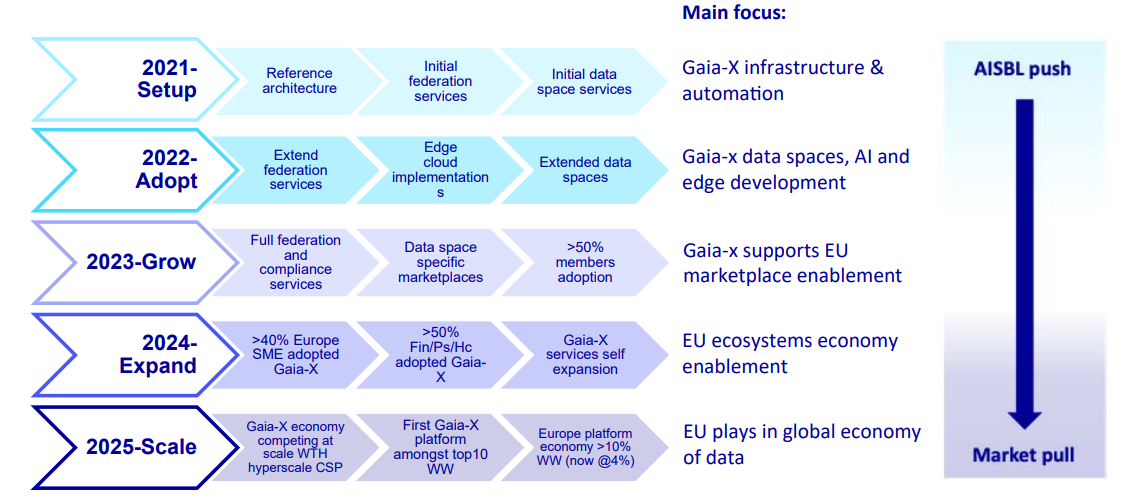
\includegraphics[width=1.1\textwidth]{gfx/chapters/6_fazit_ausblick/gaia-x-ausblick.png}
  \caption{Fünfjahresplan der Gaia-X Initiative}
  \label{fig:gaia-x-ausblick}
  \source{\cite{Bonfiglio2021}}
\end{figure}

Die Initiative Gaia-X befindet sich zur Zeit noch im Aufbau.
In \ref{fig:gaia-x-ausblick} wird der Fünfjahresplan der Initiative dargestellt.
Zum Zeitpunkt der Arbeit läuft die erste Phase: \emph{Setup}.
Eine Implementation der aufgeführten Referenzarchitektur exisitert allerdings noch nicht.

\citeauthor{Bonfiglio2021} strebt im genannten Fünfjahresplan eine vollständige Implementierung der Föderationsservices
im Jahr 2023 an.
Durch die Enstehung eines neuen Markts soll Gaia-X 2025, in der Phase \emph{Scale},
eine Konkurrenz für Hyperscaler Clouds im globalen Markt werden \cite{Bonfiglio2021}.